\documentclass[10pt,conference]{IEEEtran}
\usepackage{graphicx}
\usepackage{amsmath}
\usepackage{cite}
\usepackage{url}
\setlength{\abovecaptionskip}{3pt}
\setlength{\belowcaptionskip}{0pt}
\setlength{\textfloatsep}{6pt}
\setlength{\intextsep}{6pt}

\begin{document}

\title{WarpDial: A Case for Reconfigurability and Explainability in Object Storage}

\author{
  \IEEEauthorblockN{Anonymous Author(s)}
  \IEEEauthorblockA{Affiliation withheld for review}
}

\maketitle

\begin{abstract}
Object storage latency is a well-known problem, and why it is so large is
rarely explained to the consumers of the storage layer. Managed
services make this abstraction possible by taking responsibility for safety,
availability, reliability, and speed; giving customers direct control over
low-level storage decisions is therefore dangerous, since a poor
configuration can compromise the guarantees the service exists to provide.
We argue explainability and reconfigurability belong in the abstraction
itself: a managed service should explain why a configuration costs what it
does. This preliminary work explores one narrow part of that goal by asking
whether per-bucket placement policies provide meaningful benefits compared
to a single global policy, and what operational overhead comes with making
placement configurable. Meeting this can require a fixed~\cite{crush2006},
parametric~\cite{mapx2020}, or content-dependent~\cite{fusion2025}
tunability layer; we explore the content-dependent case here: a
reconfigurable granularity knob that governs how an object is striped
(sharded) across storage, capable of Fusion-style~\cite{fusion2025} stripe
alignment. This is a standalone, simulated prototype, evaluated separately
on two structurally different workloads, Parquet column chunks and IVF
vector-index partitions. A dense sweep shows that the right granularity
depends on the workload. As granularity changes, byte amplification and
round trips move in opposite directions. How much this matters also
depends strongly on query selectivity. A single global default can leave
real performance on the table. The flexibility has a cost too. This
policy's location-map metadata grows with granularity. A workload-blind
default never pays that cost, but it never gets the benefit either.
\end{abstract}

\section{Introduction}

Object storage latency is a widely recognized problem. AI training,
databases, and agentic frameworks have all spent years building bespoke
client-side workarounds for it~\cite{warpdrive2026}. Object storage let
people build freely in the first place because it hid infrastructure
complexity behind a simple interface. There was no hardware to manage,
just PUT and GET. What is still unexamined is \emph{why} the latency
behind that simple interface is so large. Developers on a foundational
layer, such as a database or a filesystem, have traditionally understood
that layer well enough to reason about downstream tradeoffs. Object
storage does not offer this by design. That opacity matters more, not
less, now that agentic systems also build on top of it unattended, not
only humans. They need to reason about its behavior themselves.

That opacity is the product managed services sell. They take
responsibility for safety, availability, reliability, and speed so
customers do not have to manage the infrastructure underneath. This is why
handing customers direct control over low-level decisions is dangerous on
its own. A poor configuration can break the guarantees the service exists
to provide. More systems software is now built on top of managed services
rather than raw infrastructure. We believe explainability and
reconfigurability belong in the abstraction itself. A service should
explain why a configuration costs what it does. It should not just expose
a knob and leave a customer to guess. A bucket's SLA should be a derived
output of its policy, not an asserted number.

Part of that opacity is structural. Object stores typically apply one
placement and erasure-coding policy across an entire pool. That policy is
chosen once and stays workload-blind. The same code runs whether a bucket
holds cold backups or latency-sensitive analytics tables.
WarpDrive~\cite{warpdrive2026} responds to this. Systems software keeps
rebuilding the same primitives on top of managed storage. WarpDrive argues
these primitives belong inside the storage layer instead, tunable and
explainable, rather than leaving each side to compensate for the other's
opacity.

Custom placement policies differ most in \emph{metadata cost}.
\emph{Computed} placement derives location purely from the object key,
bucket policy, and node set, as in CRUSH-style hashing~\cite{crush2006}.
Its cost is $O(\text{buckets})$. \emph{Parametric} placement stores a
small, fixed-size record per object, such as a seed, an epoch, or a layout
version~\cite{mapx2020}. Its cost is $O(\text{objects})$, tiny and
constant. \emph{Content-dependent} placement derives the location map from
the object's own data, through bin-packing by chunk size or
content-defined chunking. Its cost is
$O(\text{objects} \times \text{units per object})$. This cost grows with
the data's own structure.

Workload-specific designs are one example of a content-dependent policy,
not the foundation this poster argues for. Fusion's~\cite{fusion2025}
file-format-aware erasure coding is one such design. It aligns stripe
boundaries to a Parquet column chunk. This nearly eliminates fragmentation,
at a cost of $\sim$1.2\% storage overhead. We generalize its bin-packing
rule into a knob. That knob is what we prototype and evaluate below.

\section{Idea \& Design}

\textbf{A content-dependent policy, concretely.} We generalize Fusion's
Algorithm 1 into a format-agnostic bin packer. The original algorithm seeds
each stripe with its largest item, then packs the rest greedily into the
least-occupied bin. Our packer takes only an arbitrary
$(\mathit{unit\_id}, \mathit{size})$ list and a stripe width $k$. It has no
format-specific logic. The computable unit is a column chunk for Parquet,
or an IVF partition for a vector index. Aligning stripes to this unit is
what makes the policy content-dependent. The location map depends on the
object's own data, not just its key.

\textbf{The knob.} A bucket's policy fixes two things. The first is the
granularity, a batch size $b$. This controls how many consecutive
finest-grained units are co-located per storage unit. $b{=}1$ never splits
a unit. $b{=}N$ collapses the bucket to one unit. The second is the EC
parameters $(k, m)$. The boundary list itself, where the units fall inside
a given object, is still supplied by the client at PUT time
(\texttt{x-warpd-computable-units: [[offset,len],...]}). That part is
content-dependent by definition, so only the client's own data can
determine it.

\textbf{Metrics in tension.} We measure three things. The first is storage
overhead versus optimal. The second is two read-side costs that pull in
\emph{opposite} directions as granularity varies: byte amplification, and
round trips, the number of distinct bins a query touches. Round trips are
our proxy for network-RTT-bound latency. The third is metadata cost, one
location-map entry per storage unit. Section~III prices this from Fusion's
own reported $\sim$8 bytes per chunk, replicated $k{+}1$-way. Finer
granularity wastes fewer bytes per bin. But it touches more bins, and
creates more metadata. Coarser granularity does the reverse.

\section{Preliminary Results}

\textbf{Setup.} We use two workloads. The first is a synthetic
TPC-H-lineitem-shaped Parquet table: 16 columns, 10 row groups, 500{,}000
rows, 160 units. The second is 500{,}000 synthetic 768-dim vectors split
into an IVF index. Partition count follows FAISS's own guidance,
$\texttt{nlist}=4\sqrt{N}$~\cite{faiss2024}, giving 2{,}828 partitions.
Partition sizes follow a Dirichlet-multinomial skew, since real IVF
clusters are unbalanced. Queries sample units uniformly by selectivity. We
use RS(9,6) erasure coding. Each point is a median over $N{=}25$ trials,
with [25th, 75th] percentile bands. We sweep three selectivity regimes,
1\%, 10\%, and 50\%, and a dense range of granularities per workload: 8
settings for Parquet, 9 for the vector index.

\textbf{Reproduction check.} FAC at Parquet column-chunk granularity reaches
\textbf{1.16\%} storage overhead versus optimal. Fusion's own paper
reports $\sim$1.2\% on their real 10\,GB file. The two numbers are the
same order of magnitude. This validates our generalized packer before we
trust anything built on top of it.

\textbf{Finding 1: the right granularity is workload-dependent, evidence a
custom bucket policy helps.} Consider batch size 16. For Parquet, this is
exactly one row group. For the vector index, it is an arbitrary batch of 16
partitions, structurally unrelated to anything in that format. At this
same batch size, Parquet's storage overhead is \textbf{79.99\%}. The vector
index's is \textbf{2.69\%}. That is a $\sim$\textbf{29.8}$\times$ gap
between two structurally different workloads. Neither cost curve predicts
the other's (Fig.~\ref{fig:overhead}). A bucket operator who hard-codes one
granularity across both workloads loses on whichever one it was not tuned
for.

\textbf{Finding 2: round trips and bytes trade off, and the size of that
tradeoff changes sharply with query selectivity.} At 50\% selectivity on
Parquet, the finest granularity costs 71.9 round trips at 23.4\% byte
overhead. The coarsest granularity costs a single round trip at 101.9\%
byte overhead. That is a $\sim$4.4$\times$ gap. At 1\% selectivity, the
same two extremes are 2.0 round trips at 114.8\% bytes versus 1.0 round
trip at 19{,}040\% bytes. That gap is $\sim$166$\times$. The byte cost of
the wrong choice grows sharply as selectivity drops. Which point is
preferable depends on whether the workload is latency-bound or
bandwidth-bound. A fixed default cannot express that distinction. A
reconfigurable one can.

\textbf{Finding 3: the operational cost of exposing this policy is concrete
and small.} We apply Fusion's own reported location-map cost, $\sim$8
bytes per chunk, replicated $k{+}1$-way. Parquet's metadata ranges from
12{,}800 bytes at the finest granularity, 160 units, down to 80 bytes at
the coarsest. The vector index's metadata ranges from 226{,}240 bytes,
2{,}828 units, down to the same 80 bytes. Computed and parametric
placement do not have this property. This policy's metadata grows directly
with how finely the knob is tuned. That is the price of the flexibility
Finding 1 shows is worth having.

\begin{figure}[t]
  \centering
  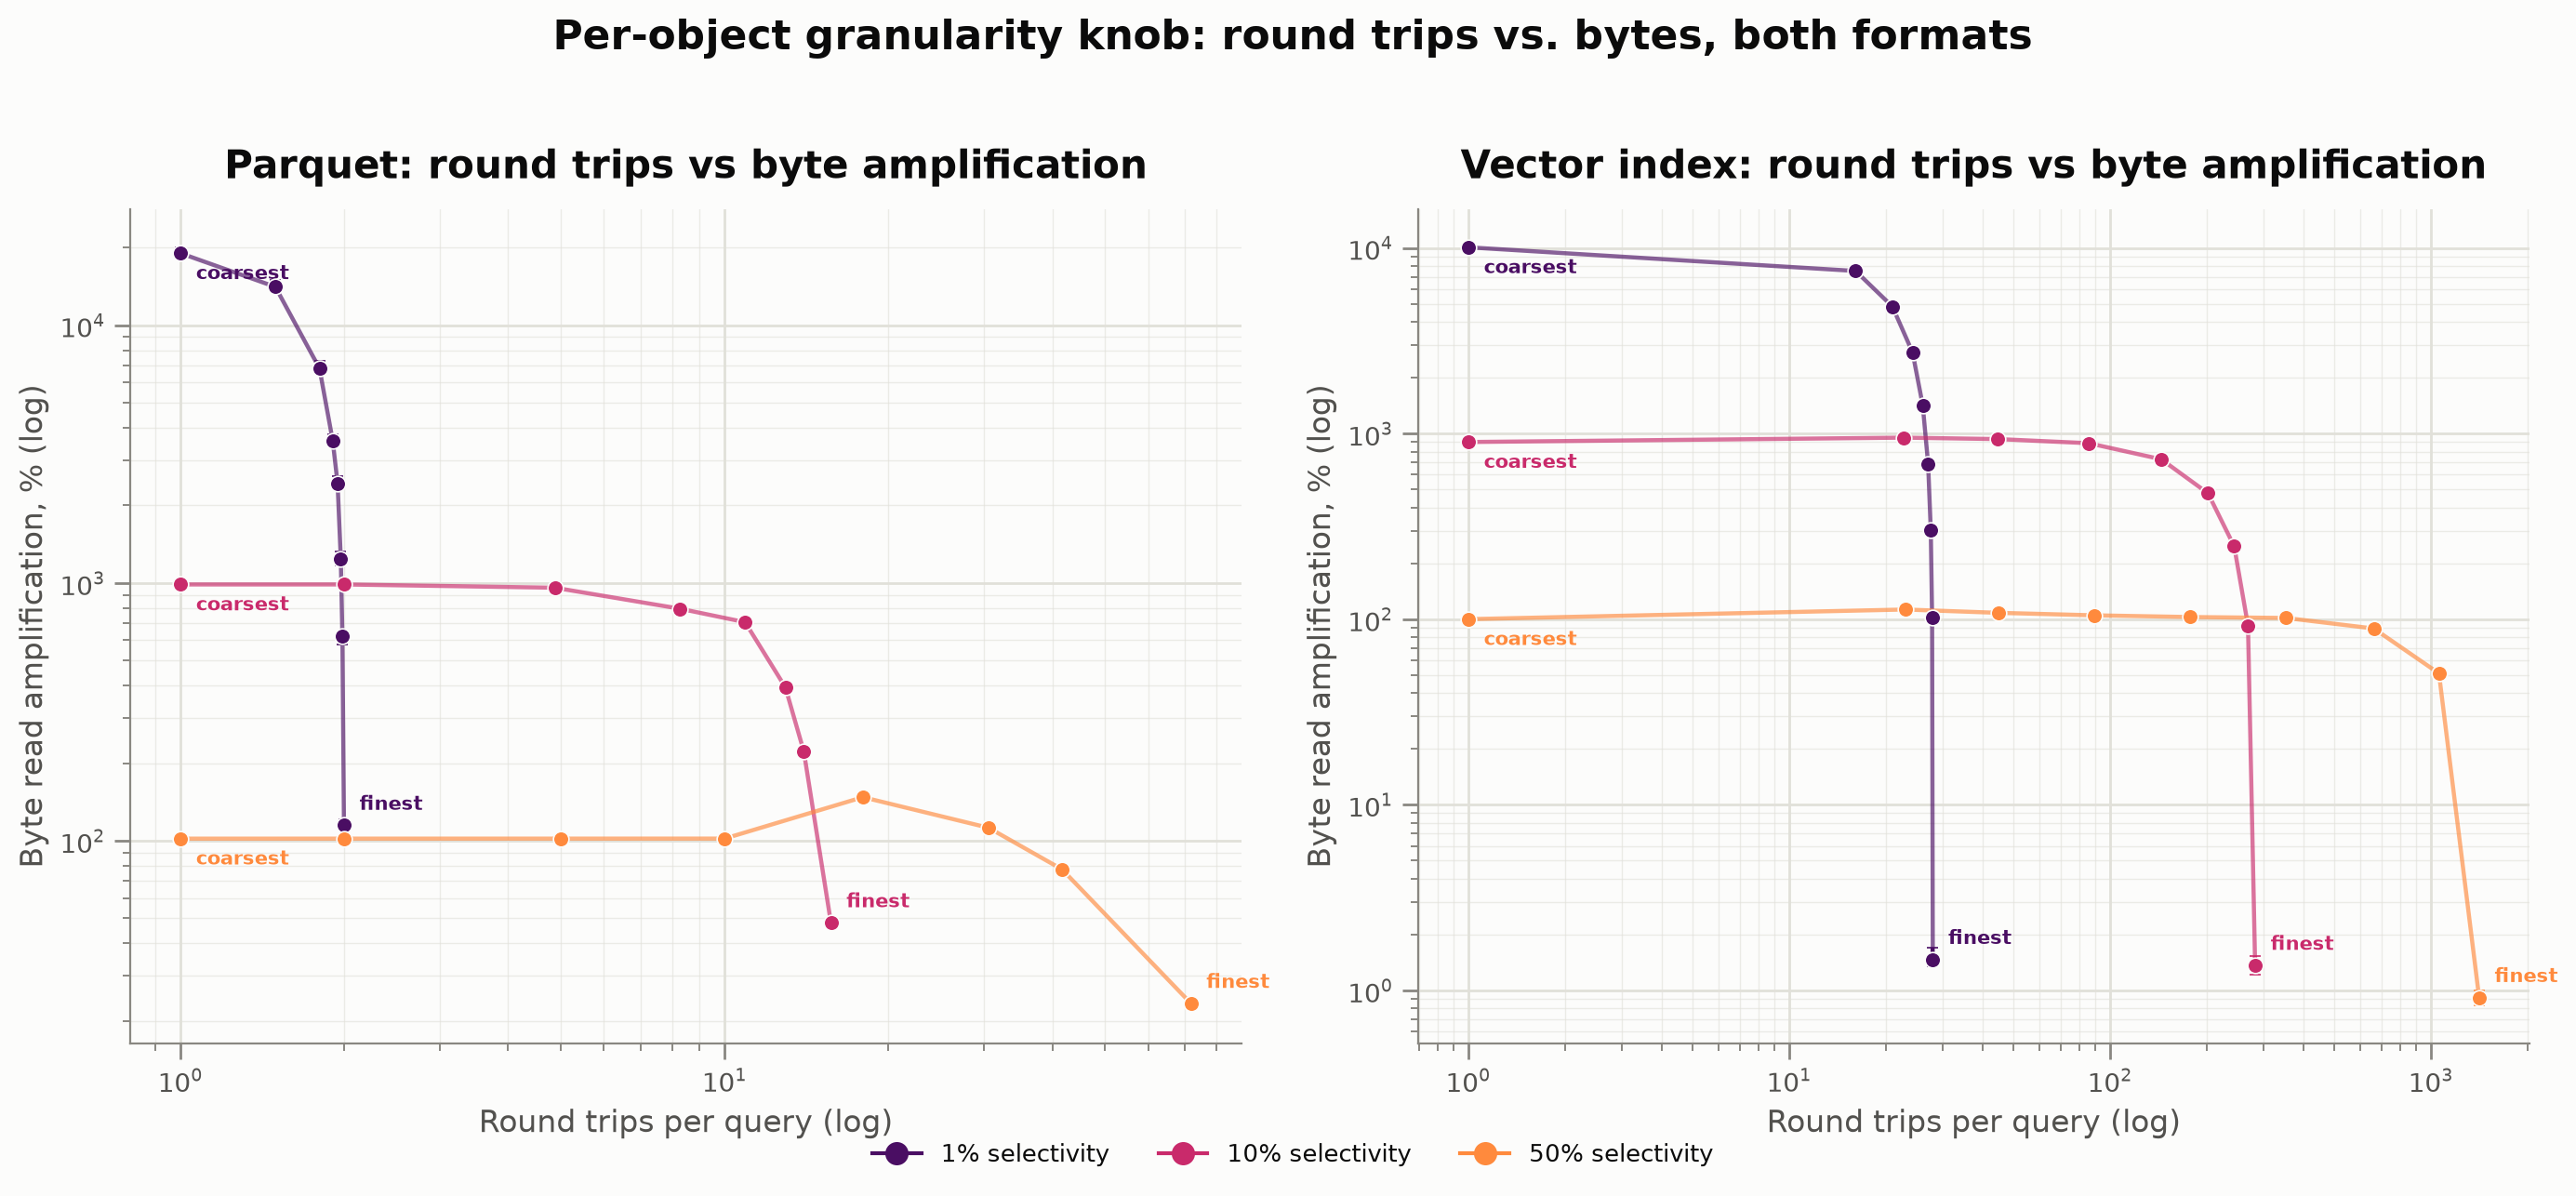
\includegraphics[width=0.62\columnwidth]{pareto_both_formats.png}
  \caption{Round trips vs.\ byte read amplification, both formats, three
  selectivity regimes. Each colored curve is the granularity-knob frontier
  (finest $\rightarrow$ coarsest) at one fixed query selectivity; selectivity
  itself is workload context, not a tuned knob, so curves are never connected
  across colors.}
  \label{fig:pareto}
\end{figure}

\begin{figure}[t]
  \centering
  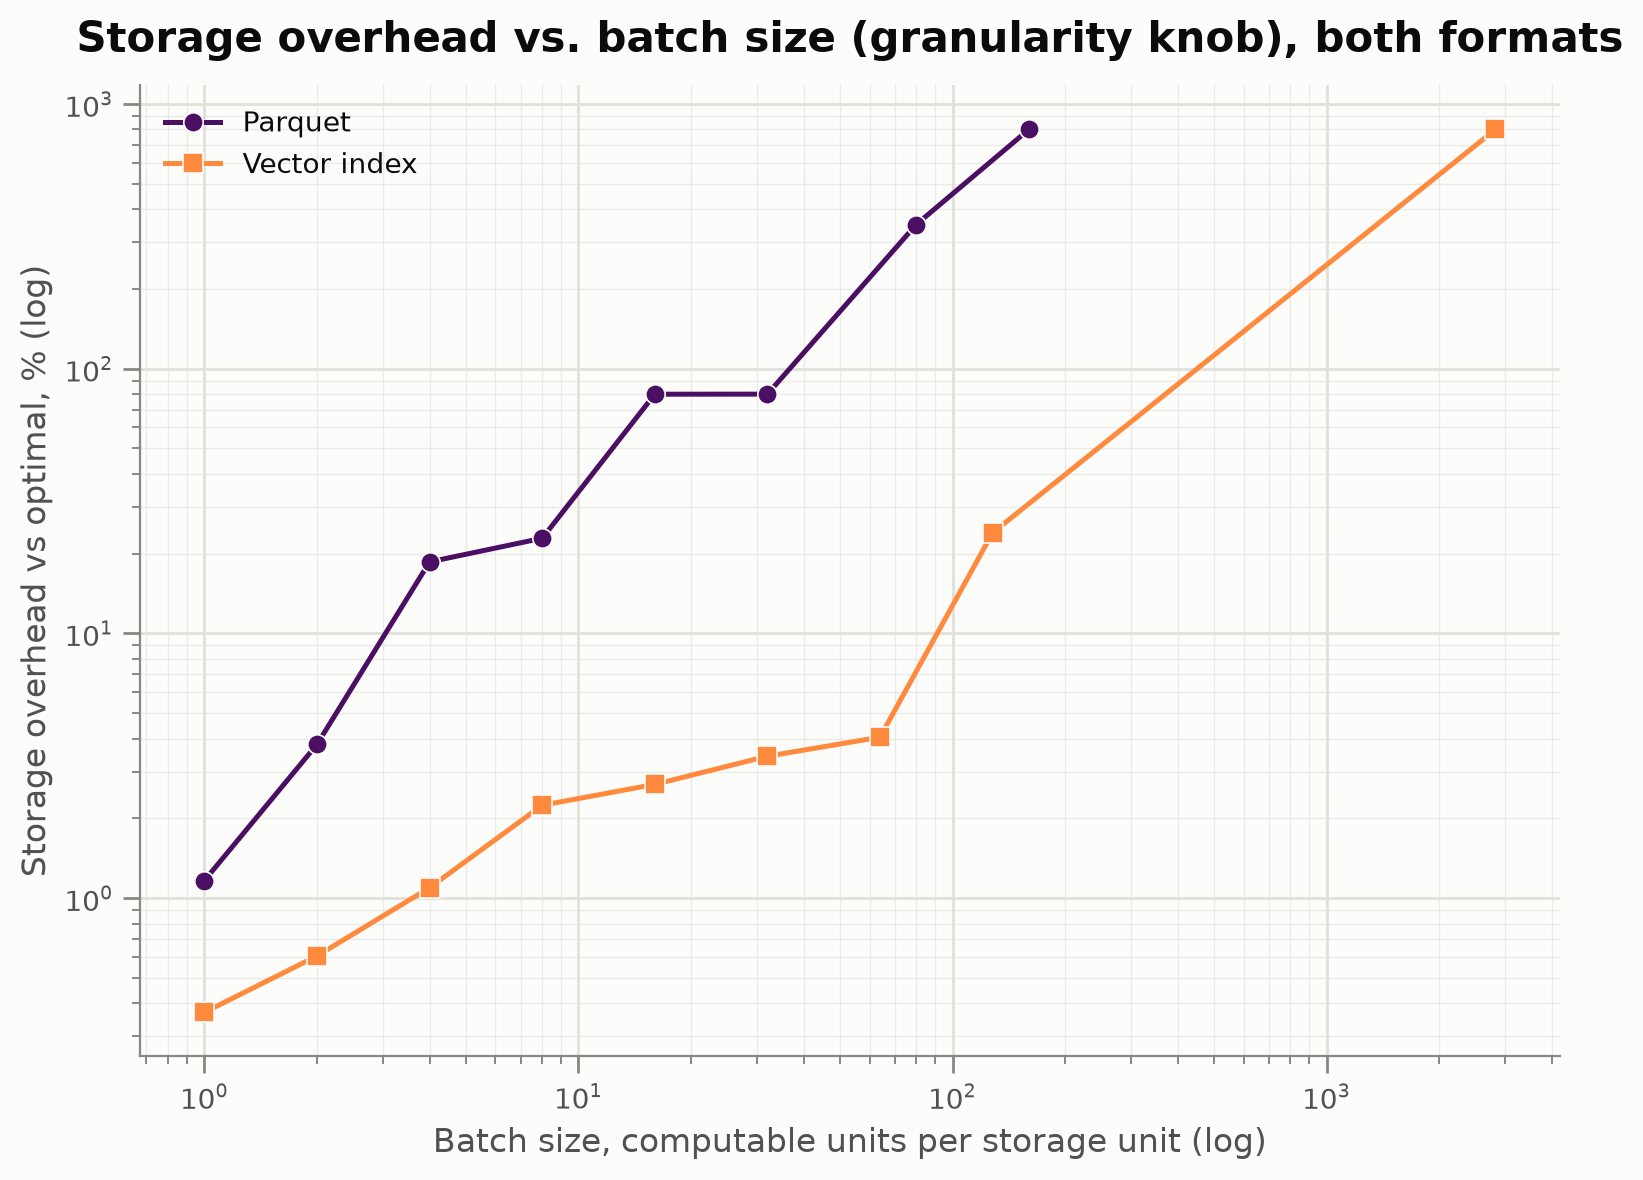
\includegraphics[width=0.46\columnwidth]{overhead_by_granularity.png}
  \caption{Storage overhead vs.\ batch size (the granularity knob), both
  formats. Overhead is a packing property, independent of query selectivity.}
  \label{fig:overhead}
\end{figure}

\section{Conclusion \& Future Work}

A managed service only earns the right to hide complexity if it can still
explain the choices it makes on a customer's behalf. We tested one
representative content-dependent policy. Letting a bucket choose its own
placement granularity helps. The right setting is workload-dependent.
Getting it wrong costs sharply more as selectivity drops, and metadata cost
rises alongside it. This is a small step toward a storage layer where
reconfigurability never costs safety. Every guarantee should be derived
and explained, not asserted. The other policy classes, SLAs as policy
outputs, and a solver over declared intents remain as future work.

{\footnotesize\section*{Acknowledgment}
Portions used AI-agent assistance, per HiPC's disclosure policy.}

{\scriptsize
\begin{thebibliography}{1}

\bibitem{fusion2025}
Y.~Lu, S.~Raina, A.~Cidon, and M.~J.~Freedman, ``Fusion: An Analytics Object
Store Optimized for Query Pushdown,'' in \emph{Proc.\ ASPLOS}, 2025.

\bibitem{warpdrive2026}
Anonymous, ``WarpDrive: A Composable Storage Substrate for Disaggregated
Data Systems,'' CDMS Workshop, VLDB 2026.

\bibitem{faiss2024}
FAISS wiki, ``Guidelines to Choose an Index.''

\bibitem{crush2006}
S.~A.~Weil et al., ``CRUSH: Controlled, Scalable, Decentralized Placement of
Replicated Data,'' in \emph{Proc.\ SC}, 2006.

\bibitem{mapx2020}
L.~Wang et al., ``MapX: Controlled Data Migration in the Expansion of
Decentralized Object-Based Storage Systems,'' in \emph{Proc.\ USENIX FAST},
2020.

\end{thebibliography}
}

\end{document}
